 
 \documentclass[11pt,a4paper]{article}

\usepackage[a4paper,bindingoffset=0.2in,%
            left=.6in,right=.7 in,top=.9in,bottom=.6in,%
            footskip=.25in]{geometry}
 
\usepackage{graphicx}
 \usepackage{amssymb}
 
\usepackage{lineno}

%\journal{Journal Name}
\begin{document}
%% Title, authors and addresses
\begin{center}
{\fontfamily{ppl}\selectfont{\large\textbf{Self-organized Simulation Model for {\textit{Dictyostelium Discoideum}}\\ Slugs Movement with Kilobots}} }
\vspace{2mm}

{\fontfamily{qbk}\selectfont\textit{Mohammad Parhizkar \\ Giovanna Di Marzo Serugendo \\ \tiny{February 2019} }}


%\vspace{2mm}
%\small{Information Systems\\Geneva School of Social Sciences \\Centre Universitaire d'Informatique\\\vspace{3mm}
%{\fontfamily{phv}\selectfont\small{Superviser: Prof. Giovanna Di Marzo Serugendo}}}
\end{center}
%% Text of abstract
\begin{abstract}
Understanding the collective behaviors in nature and its potential links to engineering the collective artificial behaviors in swarm robotics have attracted the attention among researchers. They have various impacts on different domains such as cell-biology, cancer study, the swarm of drones and unmanned robots. Since the cancer cells share similar collective behaviors, the biomedicine researchers look into different examples from nature to design anti-cancer drugs to shrink tumors in human bodies. An exciting form of collective system is demonstrated by {\textit{Dictyostelium discoideum}}. 

   \end{abstract}

{\footnotesize\textit{Keywords:} {\textit{Dictyostelium discoideum}} - Kilobot - Swarm robotics - Multi-agent systems - Self-organising systems}

{\begin{center}\noindent\rule{14cm}{0.4pt}\end{center}}
%\noindent\makebox[\linewidth]{\rule{\paperwidth}{0.2pt}}
 %% ------------------------------------------------The first section ------------------------------------------------
\section{Introduction}
The idea of simulation of slug movement in \textit{Dictyostelium discoideum} with kilobots is to have a swarm of kilobots which moves in one direction in a decentralized way, in a leader-follower manner. These robots act independently and asynchronously in the environment. 

Each slug is about $2-–4 mm$, and composed of up to $100k$ starved cells. It is capable of movement by producing a cellulose sheath around it. The slug attractants to light, heat, and humidity in a forward-only direction. Cyclic AMP and a substance called differentiation-inducing factor, help to form different cell types. In the aggregation phase of \textit{D. discoideum} cells differentiated into prestalk(pst) which is $20\%$ of the $D.~d$ population and prespore(psp) which is $80\%$ of the cells population. The pst cells move to the anterior and psp cells move to the posterior end of the slug.

We design a model of small kilobots with minimum capabilities to move to like a chain. This group of robots reaches to keep the structure of the chain by local interactions only and by utilizing positive feedback.  

In the desired chain, each kilobot needs to recognize the robot in front of it and the one behind it. This identification process happens in every time step. Interestingly, in this model we do not affiliate any id to the robots. Thus, they can move their local position in the chain intentionally. 

In this paper, we study the ...



\section {Related Works}

\section{Collective Decision-Making Model}
We design a decentralized decision-making model to allow the robots to decide between different choices, based on their neighbors in the chain. 


\section{Three Robots Distance}
 \begin{figure}[h]
     \centering
 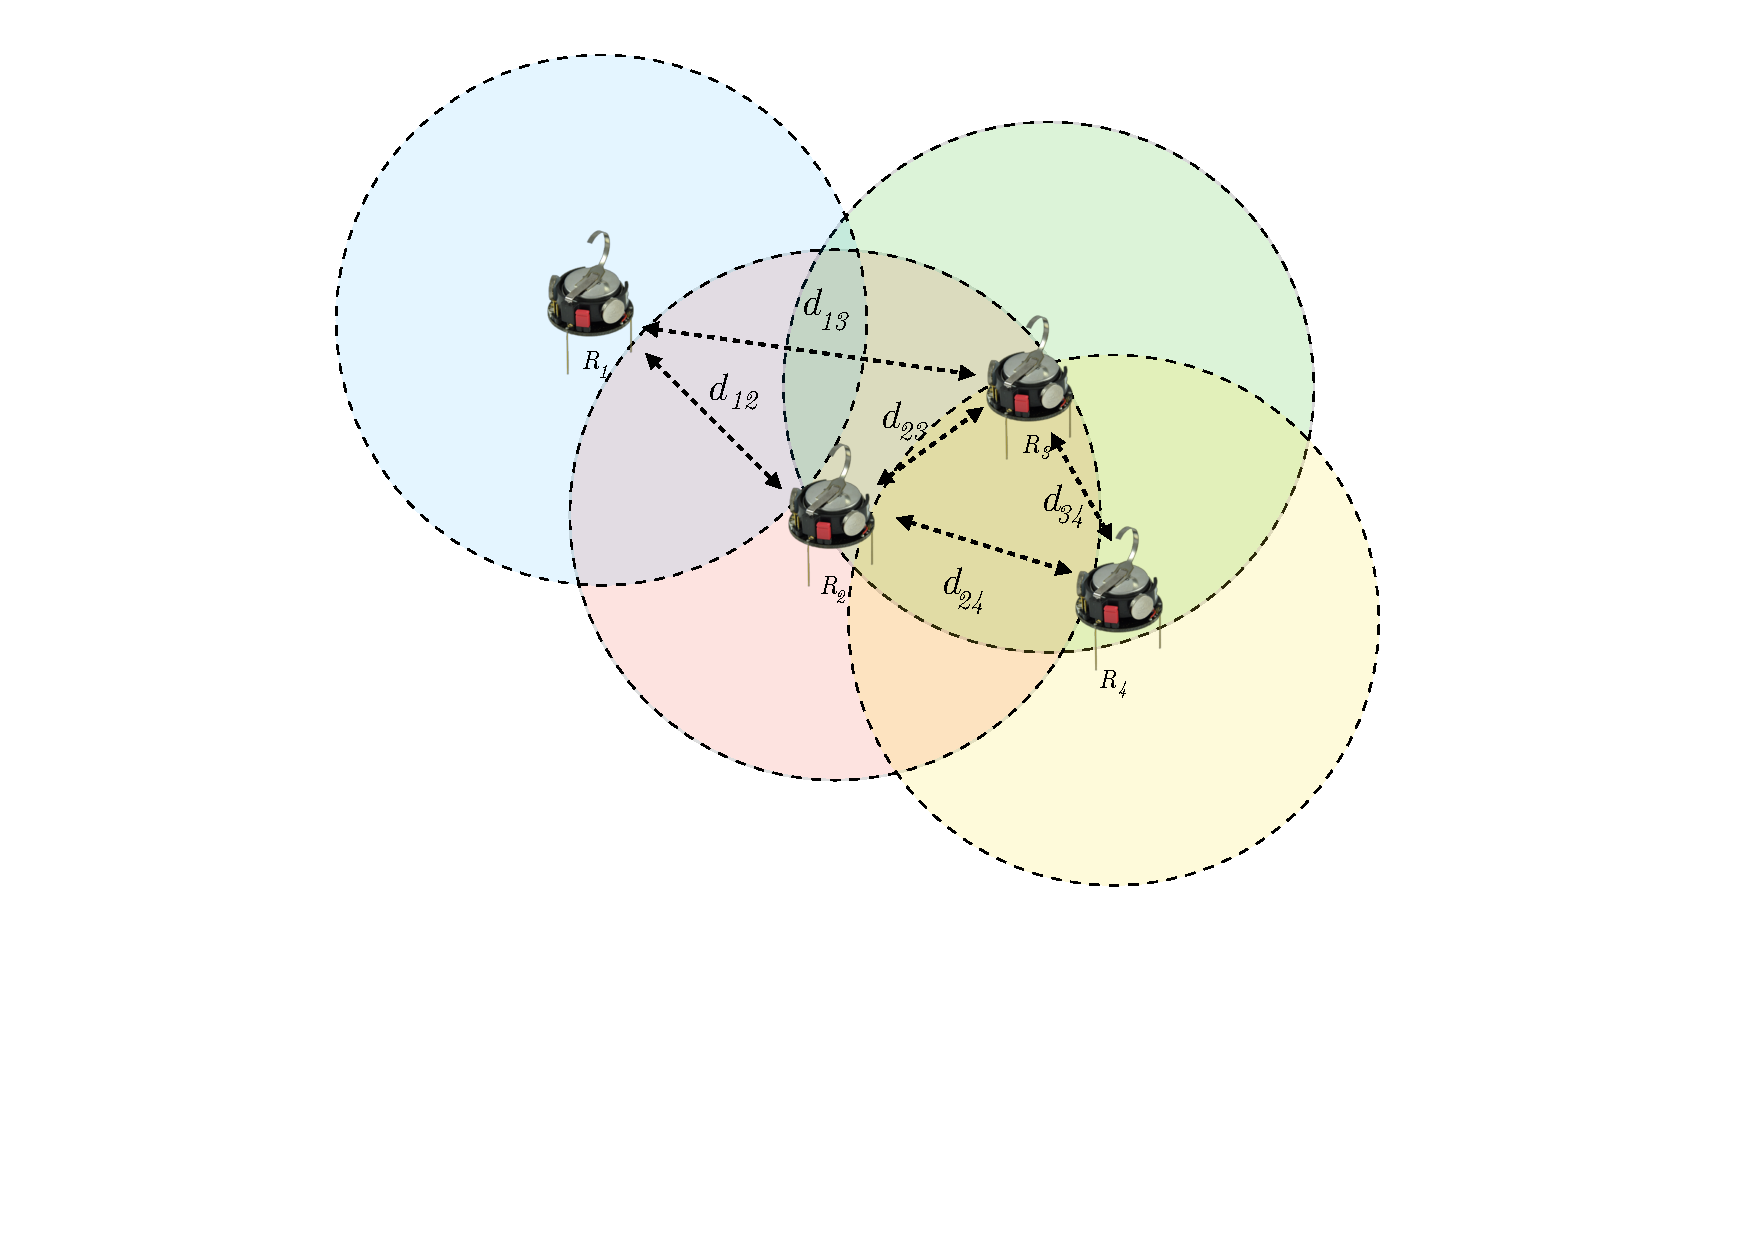
\includegraphics[scale=0.4]{Figs/PropagationArea.pdf}
     \caption{Different distances between robots and their propagation areas. }
     \label{fig:propagation}
  \end{figure}
\begin{itemize}
    \item Short-distance distance   (SD)
    \item Medium-distance distance (MD)
    \item Long-distance distance (LD) 
\end{itemize}
\section {Nine Finite Machine Scenario }
\begin{itemize}
    \item Short-distance to the leader/ Short-distance to the follower (SDLSDF)   
    \item Short-distance to the leader/ Medium-distance to the follower (SDLMDF)
    \item Short-distance to the leader/ Long-distance to the follower (SDLLDF)   
    \item Medium-distance to the leader/ Short-distance to the follower  (MDLSDF) 
    \item Medium-distance to the leader/ Medium-distance to the follower  (MDLMDF) 
    \item Medium-distance to the leader/ Long-distance to the follower (MDLLDF) 
    \item Long-distance to the leader/ Short-distance to the follower (LDLSDF) 
    \item Long-distance to the leader/ Medium-distance to the follower (LDLMDF) 
    \item Long-distance to the leader/ Long-distance to the follower (LDLLDF) 
\end{itemize}
 \section{Individual Decision Making Process }
 \begin{figure}[h]
     \centering
 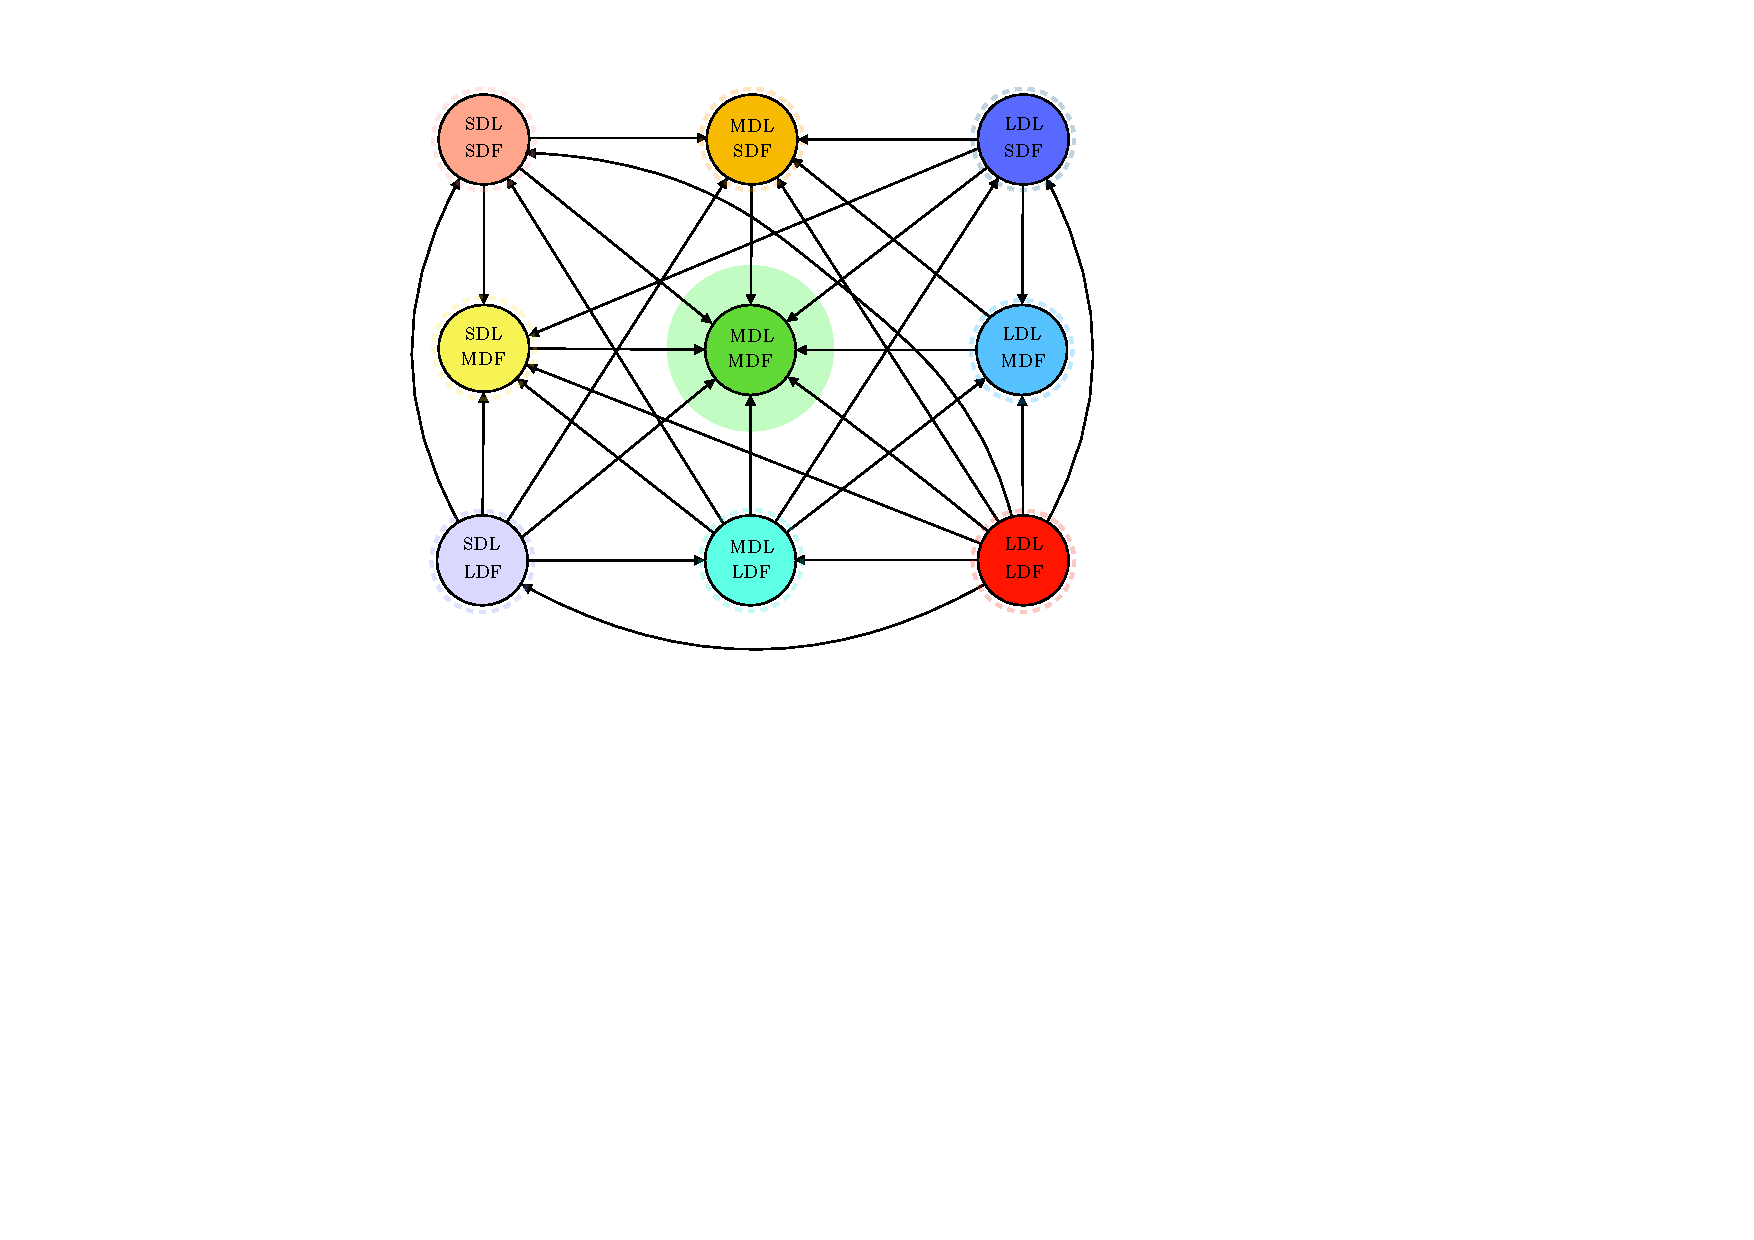
\includegraphics[scale=0.7]{Figs/States.pdf}
     \caption{Nine different states and the relationship between previous-state and current-state relationship.}
     \label{fig:states}
  \end{figure}
 
\bibliographystyle{model1-num-names}
\bibliography{sample.bib}
 

\end{document}

%%
%% End of file `elsarticle-template-1-num.tex'.